% Mở đầu

\documentclass[12pt, a4paper]{article}
\parindent 0px
\parskip=10pt
\usepackage[utf8]{vietnam}
\usepackage[left=1.20cm, right=1.20cm, top=1.50cm, bottom=1.50cm]{geometry}
\usepackage{amsmath,amssymb,amsfonts}

\usepackage{enumitem}
\usepackage{multicol}
\usepackage{graphicx}
\usepackage{array}
\usepackage{float}
\usepackage[onehalfspacing]{setspace}
\usepackage{mathpazo}
\usepackage{wrapfig}

% Title--------------------------------------------

\title{\vspace{-1.5cm}{\huge\textbf{Chuyên đề: Khảo sát hàm số}}\\[3mm]
		{\LARGE Khối lớp: 12}\\[2mm]
		{\LARGE Môn: Toán}\\[1.5mm]
{\normalsize Họ và tên~\rule{3cm}{1pt} \hfill Ngày nhận đề: ~\rule{3cm}{1pt}}\\[4mm]
\hrule
}
\author{}
\date{}

% Bắt đầu đề---------------------------------------

\begin{document}
\maketitle
\vspace{-2.25cm}

% Phần bài toán về hàm số ------------------------

\textbf{A. Bài toán về hàm số } 
\vspace{-0.25cm}

% Đơn điệu----------------------------------------

	\textbf{1. Đơn điệu}

\vspace{-0.2cm}
	
		\textbf{Câu 1: } Có bao nhiêu số nguyên $m$ để hàm số $y=(1-m)^2x^3+(m-1)x^2+x+4$ đồng biến trên $\mathbb{R}$
	
		\textbf{Câu 2: } Có bao nhiêu số nguyên $m$ để $y=\left|x^4-2x^3+mx+6-m\right|$ đồng biến trên khoảng $(0;+\infty)$
		
		\textbf{Câu 3: } Cho hàm số $f'(x)=x(x-1)(x+1).$ Khi đó hàm số $f(\sin x)$ đồng biến trên khoảng nào?
			\begin{multicols}{4}
				\begin{enumerate}
					\item[\textbf{A.}] $\left(\dfrac{3}{2};2\right)$
					\item[\textbf{B.}] $(-\infty;-10)$
					\item[\textbf{C.}] $(2;4)$
					\item[\textbf{D.}] $\left(\dfrac{8}{5};3\right)$
				\end{enumerate}
			\end{multicols}
			
		\textbf{Câu 4: } Tập hợp tất cả giá trị thực của tham số $m$ để hàm số $y=\left(\dfrac{3}{4}\right)^{x^3-3x^2+9(5-m)x+11}$ nghịch biến trên khoảng $(2;+\infty)$ là:
			\begin{multicols}{4}
				\begin{enumerate}
					\item[\textbf{A.}] $(-\infty;2)$
					\item[\textbf{B.}] $(-\infty;5)$
					\item[\textbf{C.}] $(-\infty;5]$
					\item[\textbf{D.}] $(-\infty;2]$
				\end{enumerate}
			\end{multicols}
		
		\textbf{Câu 5: } Cho hàm số $f(x)$ nhận giá trị dương trên khoảng $(1;4)$. Hàm số $f'(x)$ có bảng biến thiên sau:
		
\vspace{-0.6cm}	
	
			\begin{center}
				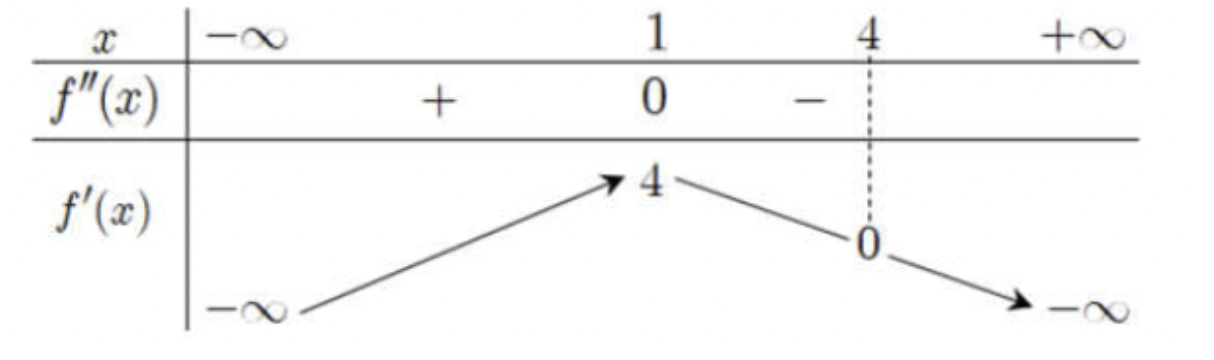
\includegraphics[scale=0.4]{../images/dondieu_cau5.png}
			\end{center}		
			
\vspace{-0.7cm}
		
		Có bao nhiêu giá trị nguyên của tham số $m \in [-20;20]$ để $g(x)=e^{mx-x^2}.f(x)$ đồng biến trên $(1;4)$?
			
		\textbf{Câu 6: } Cho hàm số $y=\dfrac{1}{3}x^3-(m+1)x^2+(m^2+2m)x-5$ với $m$ là tham số thực. Có bao nhiêu giá trị nguyên của $m\in [-2024;2024]$ để hàm số đã cho đồng biến trên khoảng $(1;5)$
		
		\textbf{Câu 7: } Cho hàm số $f(x)$ có bảng biến thiên bên dưới:
		
\vspace{-0.75cm}

			\begin{center}
				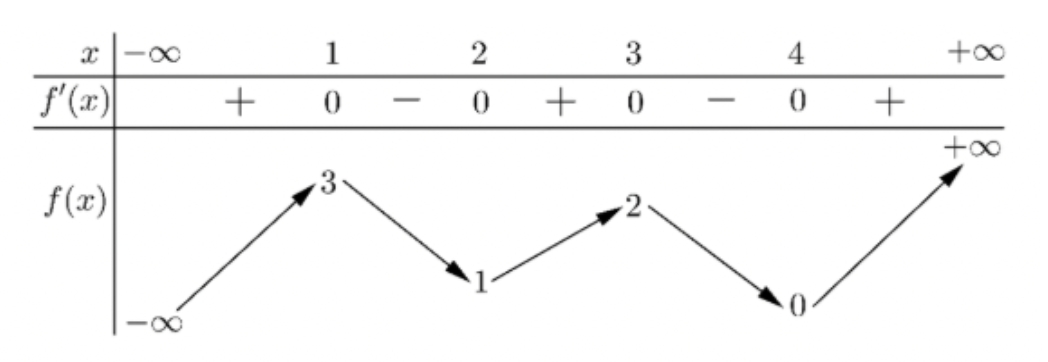
\includegraphics[scale=0.54]{../images/dondieu_cau7.png}
			\end{center}
			
\vspace{-0.8cm}			
			
		Tìm khoảng đồng biến của hàm số $y=[f(x)]^3-3[f(x)]^2$ 

\pagebreak

		\textbf{Câu 8: } Tìm $m$ để $f(x)=(m^3-2m^2-3m)x^6+(m+1)x^3+(m-1)x^2+mx$ đồng biến trên $\mathbb{R}$

		\textbf{Câu 9: } Cho hàm số $f(x)=\dfrac{1}{3}x^3-2x^2+mx+2024$ với $m$ là tham số thực. Có bao nhiêu giá trị nguyên của $m \in [-2024;2024]$ để hàm số $g(x)=f\left((x^2\right)$ đồng biến trên khoảng $(0;+\infty)$

		\textbf{Câu 10: } Có bao nhiêu giá trị của $m$ để hàm số $y=mx^9+(m^2-3m+2)x^6+(2m^3-m^2-m)x^4+m$ đồng biến trên $\mathbb{R}$

		\textbf{Câu 11*: } Cho $f(x)=2x^3+ax^2+bx+c$ có $f(0)=2f'(0)$ và $f(x) \ge 2f'(x)$ với mọi $x \ge -1$. Có bao nhiêu giá trị nguyên của $a \in (14;2024]$ để hàm số đồng biến trên $\mathbb{R}$	

		\textbf{Câu 12**: } Cho hàm số $y=f(x)$ có hàm liên tục trên $\mathbb{R}$ và đồ thị hàm số $y=f'(x)$ như hình vẽ. Có bao nhiêu giá trị nguyên của tham số $m \in [-2024;2024]$ để hàm số ${y=f(1-4x) -8mx^2+(8m+4)x+1}$ nghịch biến trên $\left(0;\dfrac{\pi}{2}\right)$
		
\vspace{-1.2cm}

			\begin{center}
				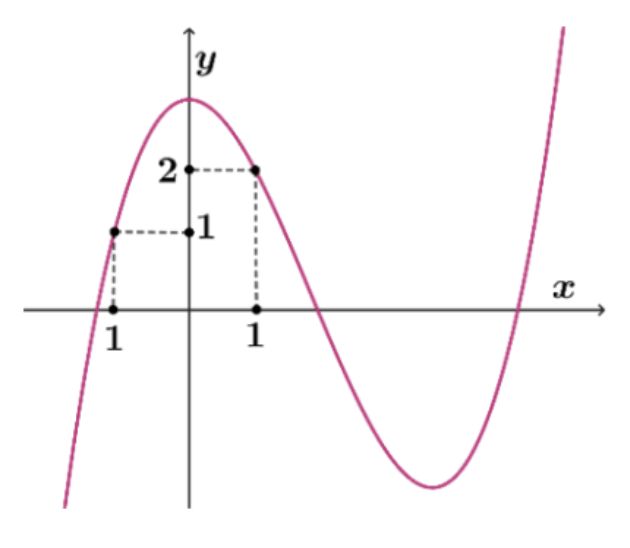
\includegraphics[scale=0.50]{../images/dondieu_cau12.png}
			\end{center}
			
\vspace{-1.2cm}

% Cực trị-----------------------------------	
				
	\textbf{2. Cực trị}
	
\vspace{-0.2cm}
	
		\textbf{Câu 1:} Hãy tìm giá trị của tham số $m$ để đường thẳng đi qua hai điểm cực trị của đồ thị hàm số $y=f(x)=\dfrac{x^2-2mx+3m-1}{x-1}$ đi qua điểm $A(3;4)$?
		
		\textbf{Câu 2: } Có bao nhiêu giá trị nguyên của tham số $m$ sao cho hàm số $y=-\dfrac{1}{3}x^3+2x^2+mx-\dfrac{4}{3}$ có đúng một điểm cực trị thuộc khoảng $(-1;8)$?
		
		\textbf{Câu 3: } Cho hàm số $y=f(x)$ có đạo hàm là $f'(x)=(x-2)^2(x^2-x), x \in \mathbb{R}$. Tìm $S$ là tập hợp các giá trị nguyên dương của tham số $m$ để $g(x)=f\left(\dfrac{1}{2}x^2-6x+m\right)$ có đúng 5 điểm cực trị.
	
		\textbf{Câu 4: } Cho hàm số $f(x)=ax^4+bx^3+cx^2+dx+e, (a \neq 0); a,b,c,d,e \in \mathbb{R}$. Hàm số $y=f'(x)$ có đồ thị $(C)$ như hình vẽ bên dưới, biết rằng $m>-e$. Số điểm cực trị của hàm số $g(x)=f'[3x-f(x)]$ là:
		
\vspace{-0.45cm}

			\begin{center}
				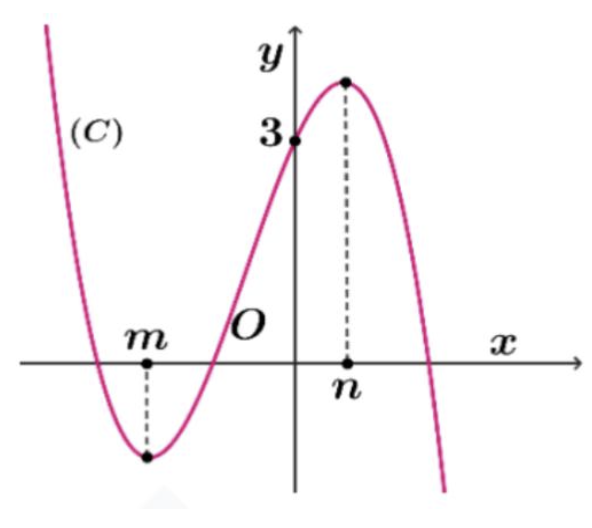
\includegraphics[scale=0.53]{../images/cuctri_cau4.png}
			\end{center}
	
\vspace{-0.8cm}		
	
		\begin{multicols}{4}
			\begin{enumerate}
				\item[\textbf{A.}] 3
				\item[\textbf{B.}] 7
				\item[\textbf{C.}] 10
				\item[\textbf{D.}] 6
			\end{enumerate}
		\end{multicols}
		
\pagebreak		
	
		\textbf{Câu 5: } Cho hàm đa thức bậc bốn, biết đồ thị $y=f'(x)$ có hai điểm cực trị là $A(0;1)$ và $B(2;5)$. Điểm cực tiểu của hàm số $g(x)=f(x)-x^2-x$ là:
		\begin{multicols}{4}
			\begin{enumerate}
				\item[\textbf{A.}] $x=0$
				\item[\textbf{B.}] $x=1$
				\item[\textbf{C.}] $x=2$
				\item[\textbf{D.}] $x=-1$
			\end{enumerate}
		\end{multicols}
		
		\textbf{Câu 6: } Cho hàm số $y=4x^3+mx^2-3x$. Có bao nhiêu giá trị của tham số $m$ để hàm số đạt cực trị tại $x_1$ và $x_2$ thỏa mãn $3x_1+x_2=1$
		
		\textbf{Câu 7: } Cho hàm số $y=-x^3+3mx^2-3m-1$ với $m \in \mathbb{R}$. Giá trị của $m$ thuộc tập hợp nào sau đây để đồ thị hàm số có hai điểm cực trị đối xứng nhau qua đường thẳng $(d):x+8y-74=0$
		
		\textbf{Câu 8*: } Cho hàm số $f(x)=\dfrac{1}{3}x^3 +mx^2+(9-m^2)x+1$. Có bao nhiêu giá trị nguyên của tham số $m$ để hàm số $y=f(|x|)$ có đúng 1 điểm cực tiểu?
		
		\textbf{Câu 9*: } Cho hàm số $y=f(x)$. Biết hàm số $y=f'(x)$ có đồ thị là đường cong trong hình bên. Có bao nhiêu giá trị nguyên dương của $m$ để hàm số $y=f\left(\left|x+\dfrac{m}{x}\right|\right)$ có đúng 6 điểm cực trị.
			\begin{center}
				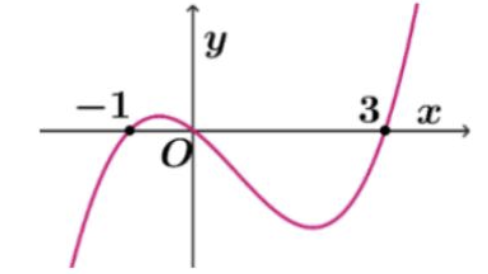
\includegraphics[scale=0.8]{../images/cuctri_cau9.png}
			\end{center}
		
		\textbf{Câu 10**: } Cho hàm số $y=f(x)=x^3-6x^2+9x-3$. Có bao nhiêu giá trị nguyên dương của $m$ để hàm số $g(x)=\left|f\left(\left|x^3+3x\right|+m-9\right)\right|$ có ít nhất 7 điểm cực trị
		
		\textbf{Câu 11***: } Cho hàm số $f(x)=x^4+mx^2-8x$ ($m$ là tham số thực). Số giá trị nguyên của $m$ để hàm số $y= \left| f \left( x^3-3x^2+2 \right) \right| $ có đúng 9 điểm cực trị
			
% GTLN - GTNN ------------------------------

\textbf{3. Giá trị lớn nhất - giá trị nhỏ nhất}

\vspace{-0.2cm}

		\textbf{Câu 1: } Cho hàm số $y=|x+m|$. Tìm $m$ để giá trị lớn nhất của $f(x)$ trên $[-2;2]$ bằng $22$.
		
		\textbf{Câu 2: } Cho hàm số $f(x)=x^3-3x^2+m$. Gọi $S$ là tập hợp các giá trị nguyên của tham số $m$ sao cho $\displaystyle\max_{\substack{[1;3]}} \left|f(x)\right| = 2 \displaystyle\min_{\substack{[1;3]}} \left|f(x)\right|$
		
		\textbf{Câu 3: } Có tất cả bao nhiêu giá trị nguyên của tham số thực $m\in [-50;50]$ để giá trị nhỏ nhất của hàm số $g(x)=\left| x^2 -(6+m)x +1 \right|$ trên khoảng $(1; +\infty)$ bằng $0$?
		
		\textbf{Câu 4: } Cho hàm số $y=f(x)$. Biết hàm số $y=f'(2-x)$ có đồ thị như hình vẽ bên dưới. Giá trị nhỏ nhất của hàm số $g(x)=f(2x-1)+2x^2-4x$ trên đoạn $\left[\dfrac{-1}{2};\dfrac{3}{2} \right]$ bằng
			\begin{multicols}{4}
				\begin{enumerate}
					\item[\textbf{A.}] $f(-1)$
					\item[\textbf{B.}] $f(-2)+\dfrac{5}{2}$
					\item[\textbf{C.}] $f(2)-\dfrac{3}{2}$
					\item[\textbf{D.}] $f(0)-\dfrac{3}{2}$
				\end{enumerate}
			\end{multicols}
			
		\textbf{Câu 5: } Cho $y=\dfrac{x+m}{x+1}$, ($m \in \mathbb{R}$) thỏa mãn. Định $m$ để $\displaystyle\max_{\substack{[1;2]}} f(x) + \displaystyle\min_{\substack{[1;2]}} f(x) = \dfrac{16}{3}$
		
		\textbf{Câu 6*: } Cho hàm số $f(x)=\dfrac{2\sqrt{x+1}+m}{\sqrt{x+1}+1}$ với $m$ là tham số. Gọi $S$ là tập hợp các giá trị nguyên của $m$ để hàm số có giá trị lớn nhất trên $[-1;8]$ nhỏ hơn 3. Số phần tử của $S$ là
		
		\textbf{Câu 7*: } Có bao nhiêu giá trị nguyên của tham số $m$ để giá trị nhỏ nhất của hàm số $f(x)=x|x+m|$ trên đoạn $[-1;2]$ không vượt quá 3?
		
		\textbf{Câu 8**:} Biết giá trị lớn nhất của hàm số $f(x)=\left|2x^3-12x^2+9x+m+8\right| + 9x$ (với $m$ là tham số) trên đoạn $[0;5]$ bằng 78. Tổng các giá trị của $m$ là?
		
		\textbf{Câu 9*: } Cho hàm số đa thức $y=f(x)$ có đồ thị như hình vẽ bên dưới. Gọi $S$ là tập hợp các giá trị của tham số $m$ để hàm số $y=\left| \left|2f(x)-6 \right| +f(x) +3 -m \right|$ có tổng giá trị lớn nhất và giá trị nhỏ nhất trên $[-1;1]$ bằng 3. Tổng các phần tử của $S$ bằng:
			\begin{center}
				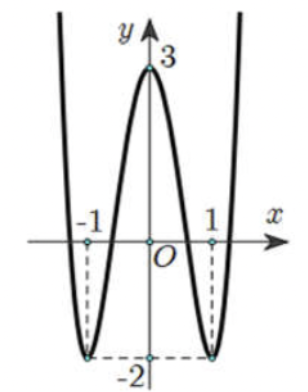
\includegraphics[scale=0.87]{../images/max_cau9.png}
			\end{center}
		\begin{multicols}{4}
			\begin{enumerate}
				\item[\textbf{A.}] 14
				\item[\textbf{B.}] 24
				\item[\textbf{C.}] 11
				\item[\textbf{D.}] 17
			\end{enumerate}
		\end{multicols}

		\textbf{Câu 10*: } Cho hàm số $f(x)$ có bảng biến thiên bên dưới. Có bao nhiêu giá trị nguyên của $m \in [-4;4]$ để hàm số $g(x)=f\left(|x^3|+|x|\right) + f(m)$ có giá trị lớn nhất trên đoạn $[-1;1]$ bằng $\dfrac{11}{2}$
			\begin{center}
				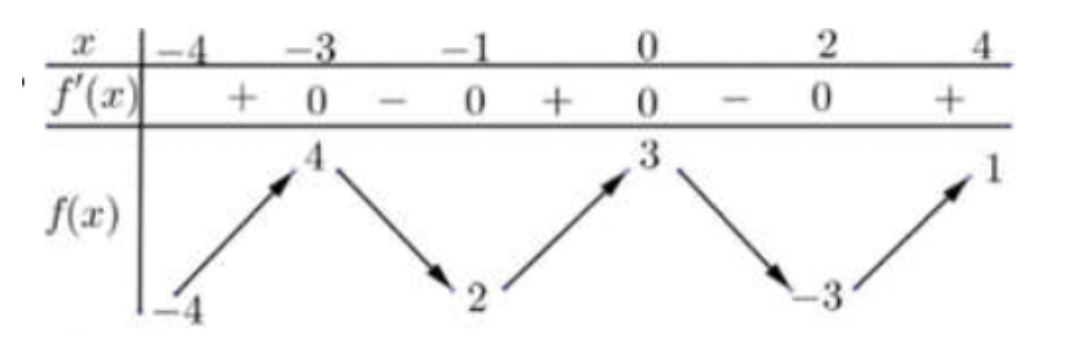
\includegraphics[scale=0.8]{../images/max_cau10.png}
			\end{center}
			
			\begin{multicols}{4}
				\begin{enumerate}
					\item[\textbf{A.}] 9
					\item[\textbf{B.}] 4
					\item[\textbf{C.}] 6
					\item[\textbf{D.}] 7
				\end{enumerate}
			\end{multicols}
			
\pagebreak

% Tiệm cận -------------------------------		
		
	\textbf{4. Tiệm cận}
	
\vspace{-0.2cm}	
	
		\textbf{Câu 1: } Cho hàm số bậc ba $f(x)$ có đồ thị như hình bên dưới. Tổng số tiệm cận đứng và tiệm cận ngang của đồ thị $g(x)=\dfrac{ x^2-x }{ [f(x)]^2-2f(x)} $ là:
		
\vspace{-0.6cm}	

			\begin{center}
				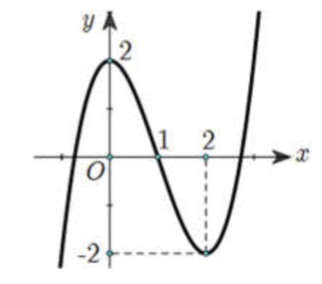
\includegraphics[scale=0.8]{../images/tiemcan_cau1.png}
			\end{center}
			
\vspace{-0.6cm}			
			
		\textbf{Câu 2: } Số đường tiệm cận của đồ thị hàm số $y=\dfrac{ \sqrt{1-x }}{ x^2-3x+2 }$ là:
		
		\textbf{Câu 3: } Cho hàm số $y=\dfrac{ mx+1 }{ x+3n+1 }$. Đồ thị hàm số nhận trục tung và trục hoành làm tiệm cận ngang và tiệm cận đứng. Khi đó $m+n$ bằng
		
		\textbf{Câu 4: } Giá trị $m$ nào dưới dây làm cho đồ thị hàm số $y=\dfrac{ 4mx+3m }{ x-2 }$ có đường tiệm cận đứng và tiệm cận ngang tạo với hai trục tọa độ một hình chữ nhật có diện tích bằng 2020?
		
		\textbf{Câu 5*: } Tìm tọa độ điểm $M$ có hoành độ dương thuộc đồ thị $(C)$ của hàm số $y=\dfrac{ x+2 }{ x-2 }$ sao cho tổng khoảng cách từ $M$ đến hai đường tiệm cận của đồ thị $(C)$ đạt giá trị nhỏ nhất.
		
		\textbf{Câu 6*: } Cho hàm số $y=\dfrac{( 2x-1 )\sqrt{mx^2-3}}{1-5x}$. Tìm $m$ để đồ thị hàm số đã cho có 1 tiệm cận xiên có hệ số góc bằng $- \dfrac{2}{5}$. Xác định phương trình tiệm cận xiện đó
		
		\textbf{Câu 7: } Cho hàm số $y=f(x)$ liên tục trên khoảng $(-\infty;1)$ và $(1;+\infty)$ có bảng biến thiên như hình bên. Tổng số đường tiệm cận của đồ thị hàm số $y=\dfrac{2^{f(x)}}{f(x)-1}$ là:
		
\vspace{-0.6cm}		
		
			\begin{center}
				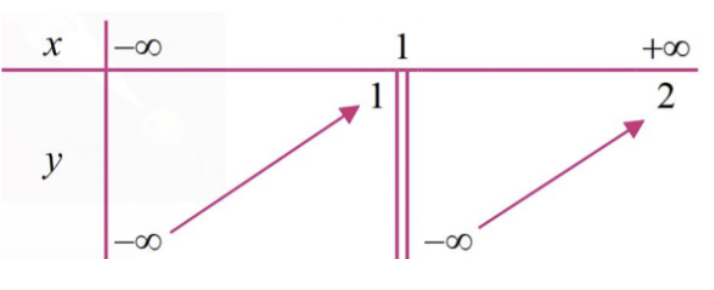
\includegraphics[scale=0.6]{../images/tiemcan_cau7.png}
			\end{center}
			
\vspace{-0.6cm}			
			
		\textbf{Câu 8**: } Cho hàm số $y=f(x)$ liên tục trên $\mathbb{R}$ và có đồ thị như hình vẽ (đồ thị hàm số nhận đường $y=0$ làm tiệm cận ngang). Số giá trị nguyên $m$ để đồ thị hàm số $y=\dfrac{22}{22\sqrt{-f(x)}+m}$ có đúng 3 đường tiệm cận
		
\vspace{-0.6cm}	
		
			\begin{center}
				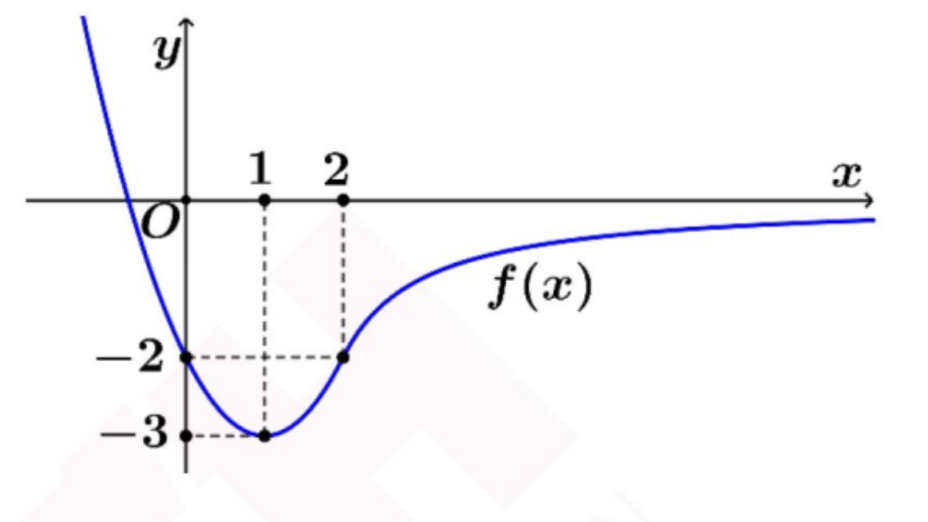
\includegraphics[scale=0.45]{../images/tiemcan_cau8.png}
			\end{center}
		
% Tương giao hàm số ---------------------------

	\textbf{5. Tương giao hàm số}
	
		\textbf{Câu 1: } Cho hàm số bậc ba $y=f(x)$ có đồ thị là đường cong trong hình bên dưới. Số nghiệm phân biệt của phương trình $f(f(x))=1$ là:

\vspace{-0.6cm}		
		
			\begin{center}
				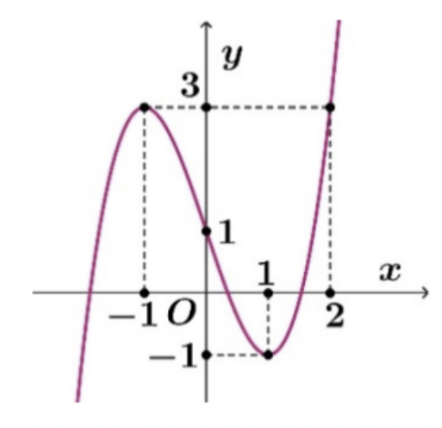
\includegraphics[scale=0.6]{../images/tuonggiao_cau1.png}
			\end{center}
			
\vspace{-0.6cm}			
			
		\textbf{Câu 2: } Cho hàm số $y=f(x)$ có đồ thị như hình bẽ bên dưới. Số nghiệm thực phân biệt của phương trình $f(x)|'f(x)|-2f'(x)=0$
		
\vspace{-0.6cm}		
		
			\begin{center}
				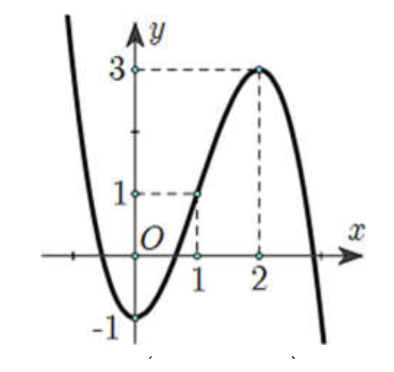
\includegraphics[scale=0.6]{../images/tuonggiao_cau2.png}
			\end{center}
			
\vspace{-0.6cm}			
			
		\textbf{Câu 3: } Cho $f(x)$ là hàm số bậc bốn. Hàm số $f'(x)$ có đồ thị như hình vẽ bên dưới. Tìm các giá trị thực của tham số $m$ để phương trình $f(e^x+1)-x-m=0$ có hai nghiệm thực phân biệt
		
\vspace{-0.6cm}	
		
			\begin{center}
				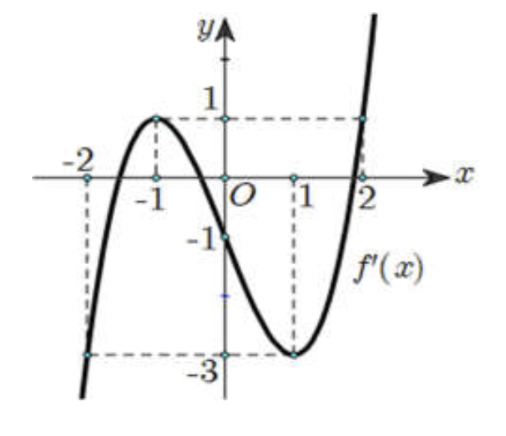
\includegraphics[scale=0.6]{../images/tuonggiao_cau3.png}
			\end{center}
			
\vspace{-0.6cm}			
			
			\begin{multicols}{4}
				\begin{enumerate}
					\item[\textbf{A.}] $m>f(2)$
					\item[\textbf{B.}] $m>f(2)-1$
					\item[\textbf{C.}] $m<f(1)-\ln 2$
					\item[\textbf{D.}] $m>f(1) + \ln 2$
				\end{enumerate}
			\end{multicols}
			
		\textbf{Câu 4: } Cho hàm số bậc ba $y=f(x)$ có đồ thị như hình vẽ bên dưới. Có bao nhiêu giá trị nguyên của tham số $m$ để phương trình $f(f(sinx))=m$ có đúng 2 nghiệm thuộc khoảng $(0;\pi)$
		
\vspace{-0.6cm}

		\begin{center}
			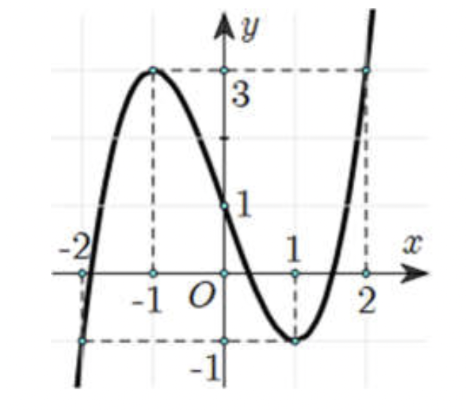
\includegraphics[scale=0.6]{../images/tuonggiao_cau4.png}
		\end{center}
		
\vspace{-0.6cm}

		\textbf{Câu 5: } Cho hàm số bậc ba $f(x)$ có đồ thị như hình vẽ bên. Tìm các giá trị của tham số $m$ để phương trình $[f(x)]^2+(m-1)f(x)=0$ có đúng 4 nghiệm phân biệt?
		
\vspace{-0.6cm}		
		
			\begin{center}
				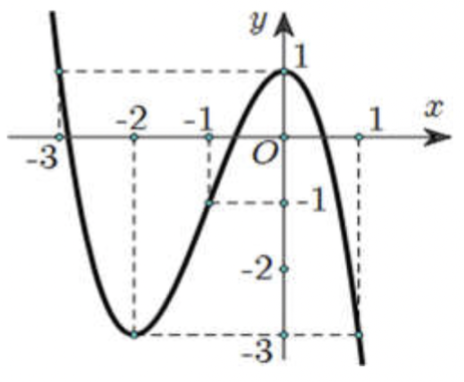
\includegraphics[scale=0.6]{../images/tuonggiao_cau5.png}
			\end{center}

\vspace{-0.6cm}
				
		\textbf{Câu 6: } Cho hàm số $f(x)=x^3-3x^2+1$ có đồ thị như hình vẽ bên dưới. Phương trình $\dfrac{f(f(x))+1}{f(x)-1}=1$ có tất cả bao nhiêu nghiệm

\vspace{-0.6cm}

			\begin{center}
				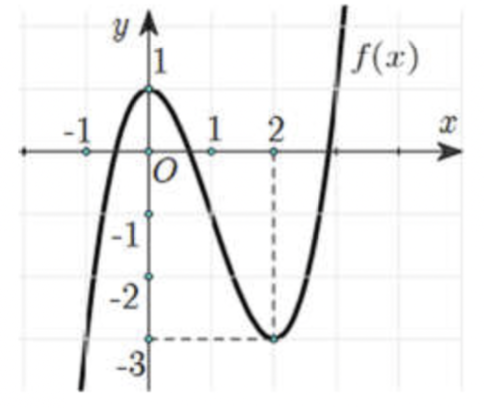
\includegraphics[scale=0.6]{../images/tuonggiao_cau6.png}
			\end{center}
			
\vspace{-0.6cm}
			
		\textbf{Câu 7: } Cho hàm số $y=f(x)$ có bảng biến thiên bên dưới. Số nghiệm thực phân biệt của phương trình $f \left(\left(f(x)\right)^2\right)-4=0$
		
\vspace{-0.6cm}
		
			\begin{center}
				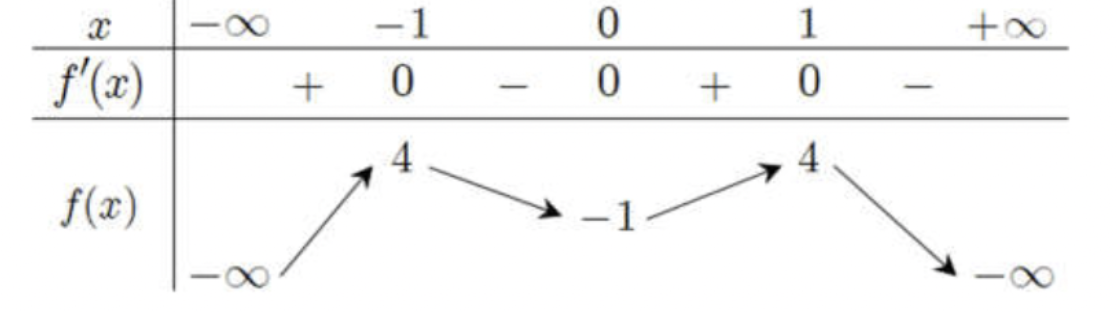
\includegraphics[scale=0.6]{../images/tuonggiao_cau7.png}
			\end{center}
			
\vspace{-0.6cm}		

		\textbf{Câu 8**: } Cho hàm số $y=f(x)$ liên tục trên $\mathbb{R}$ và có bảng biến thiên như hình sau:
		
\vspace{-0.6cm}	
	
			\begin{center}
				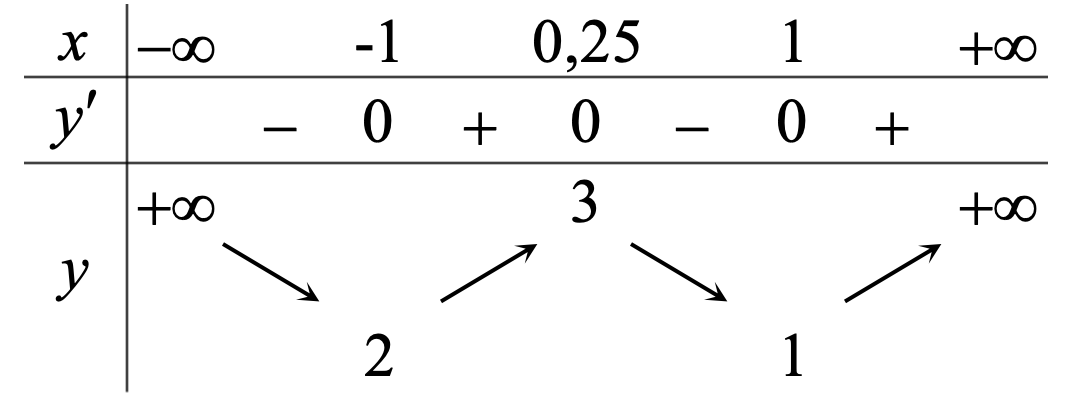
\includegraphics[scale=0.5]{../images/tuonggiao_cau9.png}
			\end{center}
			
\vspace{-0.6cm}
			
		Có bao nhiêu giá trị nguyên của tham số $m$ để bất phương trình có nghiệm đúng $\forall x \in \mathbb{R}$: $$2.6^{f(x)} +\left(f^2(x)-1\right).9^{f(x)} -3.4^{f(x)}.m \geq (2m^2+2m).2^{f(x)}$$ 
		
		\textbf{Câu 9**: } Cho hàm số $f(x)=x^4-32x^2+4$. Có bao nhiêu giá trị nguyên của tham số $m$ sao cho ứng với mỗi $m$, tổng giá trị các nghiệm phân biệt thuộc khoảng $(-4;1)$ của phương trình $f(x^2+4x+5)=m$ bằng $-8$.
			
\pagebreak			
			
% Phương trình tiếp tuyến ---------------------

	\textbf{6. Phương trình tiếp tuyến (Mức độ: "khó" đến "rất khó" đến "trang trí" )}
		
\vspace{-0.2cm}

		\textbf{Câu 1*: } Cho hai hàm số $f(x)=\dfrac{1}{x\sqrt{2}}$ và $g(x)=\dfrac{x^2}{\sqrt{2}}$. Gọi $d_1$,$d_2$ lần lượt là tiếp tuyến của mỗi đồ thị hàm số $f(x)$, $g(x)$ đã cho tại giao điểm của chúng. Hỏi góc giữa hai tiếp tuyến trên bằng bao nhiêu?
		
		\textbf{Câu 2**: } Cho hàm số $y=f(x)=\dfrac{x^4}{4}-x^2$ có đồ thị $(C)$. Gọi $M(m;f(m)$ là điểm thuộc $(C)$ sao cho tiếp tuyến tại $M$ của $(C)$ cắt $(C)$ tại hai điểm phân biệt $A$ và $B$ sao cho $MA=3MB$. Tìm tất cả các giá trị $m$.
		
		\textbf{Câu 3**: } Trong mặt phẳng $Oxy$, có bao nhiêu điểm mà từ đó kẻ được hai tiếp tuyến đến đồ thị hàm số $y=\dfrac{1}{3}x^3-\dfrac{1}{2}x^2+x+1$ sao cho tiếp tuyến này vuông góc với nhau?
		
		\textbf{Câu 4*: } Cho hàm số $y=\dfrac{x-2}{x+1}$ có đồ thị là $(C)$ và $I(-1;1)$. Tiếp tuyến $\Delta$ của $(C)$ cắt hai đường tiệm cận của đồ thị hàm số $(C)$ lần lượt tại $A;B$ sao cho chu vi tam giác $IAB$ đạt giá trị nhỏ nhất. Khi đó chu vi nhỏ nhất của tam giác $IAB$
		
		\textbf{Câu 5**: } Cho hàm số $f(x)=x^3+3x^2+mx+1$. Gọi $S$ là tổng tất cả giá trị của tham số $m$ để đồ thị hàm số $y=f(x)$ cắt đường thẳng $y=1$ tại ba điểm phân biệt $A(0;1), B, C$ sao cho các tiếp tuyến của đồ thị hàm số $y=f(x)$ tại $B,C$ vuông góc với nhau. Giá trị của $S$ bằng
		
		\textbf{Câu 6***: } Một tiếp tuyến của đường cong $y^2-x^2=1$ cắt hai đường thẳng $y=x,y=-x$ tại $A$ và $B$. Tính diện tích tam giác $OAB$.
		
		\textbf{Câu 7*: } Tìm $m$ để đồ thị hàm số $y=x^3-3x^2+mx-m$ cắt trục hoành tại 3 điểm phân biệt $A,B,C$ sao cho tổng hệ số góc của các tiếp tuyến với đồ thị hàm số tại các điểm $A,B,C$ bằng 3.
		
		\textbf{Câu 8***: } Cho hàm số $f(x)=\dfrac{1}{2}x^2-mx$ và $g(x)=\dfrac{x-m}{x-1}$, tham số $m\neq1$, có đồ thị $(C_1)$,$(C_2)$. Biết rằng tồn tại đúng 2 số $x_0 \in (2;3)$ sao cho nếu gọi $d_1$, $d_2$ là tiếp tuyến tại các điểm có hoành độ $x_0$ thuộc $(C_1)$,$(C_2)$ và $d_1$,$d_2$ cắt nhau tại $A$, còn $d_1$, $d_2$ cắt trục $Ox$ ở $B$,$C$ thì $AB=AC$. Tìm tất cả các giá trị $m$.
		
		\textbf{Câu 9**: } Cho hàm số $y=(x^2-1)^2$ có đồ thị $(C)$. Xét điểm $M$ di chuyển trên $(C)$ và có hoành độ $m\in (-1;1)$. Tiếp tuyến của $(C)$ ở $M$ cắt $(C)$ tại hai điểm $A$, $B$ phân biệt và khác $M$. Tìm giá trị lớn nhất của tung độ trung điểm $I$ của đoạn thẳng $AB$.
		
		\textbf{Câu 10**: } Cho các hàm số $y=f(x)$, $y=f\left[f(x)\right]$, $y=f\left( \sqrt{x^2+24} \right)$ có đồ thị lần lượt là $(C_1)$,$(C_2)$,$(C_3)$. Đường thẳng $x=1$ cắt $(C_1)$,$(C_2)$,$(C_3)$ lần lượt tại các điểm $M$, $N$, $P$. Biết phương trình tiếp tuyến của $(C_1)$ tại $M$ và của $(C_2)$ tại $N$ lần lượt tại $y=2x+3$ và $y=202(10x+1)$. Viết phương trình tiếp tuyến của $(C_3)$ tại $P$. 
		
		\textbf{Câu 11***: } Cho hàm số $y=x+\dfrac{1}{x}$ $(x>0)$ có đồ thị $(C)$. Tìm tập hợp các điểm trong mặt phẳng mà từ đó có thể kẻ đúng hai tiếp tuyến đến $(C)$ sao cho đường thẳng nối hai tiếp điểm luôn đi qua điểm $I(1;1)$
		
\end{document}
